\chapter{Algoritmo di Thomas}

L'algoritmo di Thomas è un metodo numerico molto efficiente per la risoluzione di sistemi lineari la cui matrice dei coefficienti è \textbf{tridiagonale}. Questo tipo di sistemi compare frequentemente nella discretizzazione di equazioni differenziali mediante metodi alle differenze finite.

Consideriamo dunque il seguente sistema di equazioni lineari:

\[\begin{aligned}
	v_1 \phi_1\, +\, &w_1 \phi_2\, \quad \quad \quad =\, S_1 \\
	u_2 \phi_1\, +\, &v_2 \phi_2 + w_2 \phi_3 \quad \quad =\, S_2 \\
	\dots \ \ &u_3 \phi_2 + v_3 \phi_3 + w_3 \phi_4\, =\, S_3 \\
	&\ \cdots
\end{aligned}\]

dove $u_i$ rappresentano i coefficienti sotto la diagonale principale, $v_i$ rappresentano i coefficienti sulla diagonale principale, $w_i$ rappresentano i coefficienti sopra la diagonale principale, $S_i$ rappresentano i termini noti del sistema.

\subsection*{Eliminazione della prima variabile}

Il primo passo dell'algoritmo consiste nell'eliminare progressivamente le variabili procedendo lungo il sistema.

Si sottrae la seconda equazione, moltiplicata per $v_1$, dalla prima moltiplicata per $u_2$.

Successivamente si procede a normalizzare le equazioni dividendo la prima equazione per $v_1$ e la seconda per $(v_2 v_1 - u_2 w_1)$.

In questo modo si ottiene un sistema equivalente nel quale i coefficienti delle variabili $\phi_1$ e $\phi_2$ risultano normalizzati a uno:

\[ \begin{aligned}
	\phi_1 + \frac{w_1}{v_1}&\phi_2 \qquad \qquad \qquad\ \ \ =  \frac{S_1}{v_1} \\
	&\phi_2 + \frac{w_2 v_1}{(v_2 v_1 - u_2 w_1)} \phi_3
	=
	\frac{S_2 v_1 - S_1 u_2}{(v_2 v_1 - u_2 w_1)}\\
	u_3 &\phi_2 + v_3 \phi_3 + w_3 \phi_4 \quad\ \ \ = S_3
\end{aligned} \]

\subsubsection*{Riscrittura del sistema}

Le espressioni precedenti possono essere riscritte in una forma più compatta osservando che $\frac{w_2 v_1}{v_2 v_1 - u_2 w_1}=\frac{w_2}{v_2 - u_2 \frac{w_1}{v_1}}$ e analogamente per il termine noto $\frac{S_2 - S_1 u_2/v_1}{(v_2 - u_2 w_1/v_1)}$.

Il sistema diventa quindi:

\[ \begin{aligned}
	\phi_1 + \frac{w_1}{v_1}\phi_2 &= \frac{S_1}{v_1} \\
	\phi_2 +
	\frac{w_2}{\left(v_2 - u_2 \frac{w_1}{v_1}\right)} \phi_3
	&=
	\frac{S_2 - S_1\frac{u_2}{v_1}}
	{\left(v_2 - u_2 \frac{w_1}{v_1}\right)}\\
	u_3 \phi_2 + v_3 \phi_3 + w_3 \phi_4 &= S_3
\end{aligned}\]

\subsubsection*{Introduzione dei coefficienti ricorsivi}

A questo punto è conveniente introdurre nuovi coefficienti che permettono di riscrivere il sistema in forma ricorsiva.

Definiamo:

\[\alpha_1 = \frac{w_1}{v_1}\ \ ,\qquad \qquad 
\beta_1 = \frac{S_1}{v_1}\]

e successivamente:

\[ \alpha_2 = \frac{w_2}{(v_2 - u_2 \alpha_1)}\ \ , \quad \quad \beta_2 = \frac{S_2 - u_2 \beta_1}{(v_2 - u_2\alpha_1)}\]


Utilizzando queste definizioni il sistema assume la forma

\[\begin{aligned}
	\phi_1 + \alpha_1 \phi_2 &= \beta_1 \\
	\phi_2 + \alpha_2 \phi_3 &= \beta_2 \\
	u_3 \phi_2 + v_3 \phi_3 + w_3 \phi_4 &= S_3\\
	\ \ \dots
\end{aligned}\]

\subsection*{Passo ricorsivo}

Il procedimento può essere ripetuto anche per le equazioni successive.
Si sottrae dall'ultima equazione scritta la precedente moltiplicata per $u_3$, poi si divide il risultato per il coefficiente di $\phi_3$. Si ottiene:

\[\phi_3 + \frac{w_3}{v_3 - u_3 \alpha_2}\phi_4 =
\frac{S_3 - u_3 \beta_2}{v_3 - u_3 \alpha_2}\]

Confrontando questa espressione con le definizioni precedenti si osserva che è possibile introdurre una definizione ricorsiva generale dei coefficienti.

Per $i=2,\dots,N$:

\begin{align}
	\alpha_i &=
	\frac{w_i}{(v_i - u_i \alpha_{i-1})}
	\tag{16}\\
	\beta_i &=
	\frac{S_i - u_i \beta_{i-1}}
	{(v_i - u_i \alpha_{i-1})}
	\tag{17}
\end{align}

Queste relazioni permettono di determinare progressivamente tutti i coefficienti $\alpha_i$ e $\beta_i$.

\subsection*{Forma finale del sistema}

Dopo aver applicato questo procedimento a tutte le equazioni del sistema, assume la forma

\[\begin{aligned}
	\phi_1 &= \beta_1 - \alpha_1 \phi_2 \\
	\phi_2 &= \beta_2 - \alpha_2 \phi_3 \\
	\cdots \\
	\phi_{N-1} &= \beta_{N-1} - \alpha_{N-1} \phi_N \\
	\phi_N &= \beta_N
\end{aligned}\]

L'ultima equazione fornisce immediatamente il valore di $\phi_N$.

Una volta noto $\phi_N$ è possibile determinare tutte le altre incognite tramite una procedura di sostituzione all'indietro: $\phi_{N-1}, \phi_{N-2}, \dots, \phi_1$ .


\subsection*{Costo computazionale}


Il numero di operazioni in virgola mobile (floating point operations, FLOP) richiesto dall'algoritmo di Thomas per risolvere un sistema lineare di $N$ equazioni è $\boxed{\, 10N - 11\, }$ .

Questo significa che il costo computazionale cresce linearmente con la dimensione del sistema.


\begin{multicols}{2}
\subsection*{Prestazioni}

Consideriamo ad esempio un processore in grado di eseguire 600 \text{ GFLOPS} cioè $600 \times 10^9$.

operazioni floating point al secondo (come ad esempio il processore AMD Ryzen Threadripper 2990WX).

In queste condizioni il tempo necessario per risolvere un sistema lineare con $N = 1000$ equazioni è dell'ordine di $17 \text{ ns}$ .


\begin{figure}[H]
	\label{ryzen}
	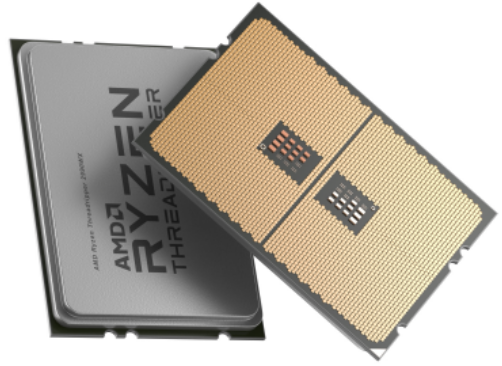
\includegraphics[width=6cm]{img/ryzen.png}
	\caption{catzo e palle}
\end{figure}

\end{multicols}